\begin{figure*}[!t]
\centering
\input{figures/evaluation-marks}
\begin{minipage}[t]{0.405\textwidth}
\raggedright\small
\textbf{A. The input reverses the model ranking}\par
\smallskip
Both models score the token under the outlined mask after the same prefix. Points show next-token loss in bits per byte (lower is better).\par
\medskip
\centering
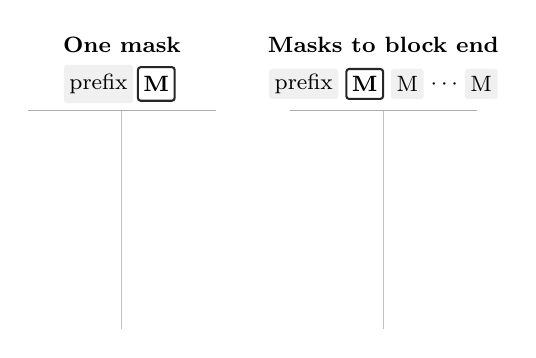
\begin{tikzpicture}[x=1cm,y=1cm,font=\small,
  token/.style={fill=black!6,rounded corners=1pt,minimum height=.38cm,inner xsep=2pt,font=\footnotesize},
  target/.style={token,draw=black!85,fill=white,line width=.75pt,font=\bfseries\footnotesize}]
\def\one{1.30}
\def\many{4.62}
% Each input heads one column. The guide passes through both measurements.
\foreach \x/\heading in {\one/One mask,\many/Masks to block end}{
  \node[font=\bfseries\footnotesize] at (\x,3.63) {\heading};
  \draw[black!32] ({\x-1.19},2.79)--({\x+1.19},2.79);
  \draw[black!24] (\x,2.79)--(\x,.02);}
\node[token,anchor=east] at ({\one+.15},3.13) {prefix};
\node[target,anchor=west] at ({\one+.19},3.13) {M};
\matrix[column sep=2.5pt,inner sep=0pt,ampersand replacement=\&] at (\many,3.13) {
  \node[token] {prefix}; \& \node[target] {M}; \& \node[token] {M}; \&
  \node[font=\footnotesize] {$\cdots$}; \& \node[token] {M}; \\
};
\def\noiseline#1#2#3#4#5#6{
  \coordinate (first) at (\one,{.15+5.65*(#5-1.30)});
  \coordinate (last) at (\many,{.15+5.65*(#6-1.30)});
  \draw[#1,thick,#2] (first)--(last);
  \foreach \point in {first,last}{\node[shape=#3,fill=#1,inner sep=0pt,minimum size=4pt] at (\point) {};}
  \node[left=4pt,text=#1,inner sep=0pt] at (first) {#5};
  \node[right=4pt,text=#1,inner sep=0pt] at (last) {#6};
  \node[anchor=west,xshift=4pt,#4,text=#1,inner sep=0pt,font=\footnotesize] at (first) {\modelname};}
\def\fixednoise#1#2{\def\modelname{Fixed noise range}\noiseline{black!75}{dashed}{rectangle}{yshift=-.47cm}{#1}{#2}}
\def\calibratednoise#1#2{\def\modelname{Calibrated range}\noiseline{blue!75!black}{solid}{circle}{yshift=.10cm}{#1}{#2}}
\drawnoise
\end{tikzpicture}
\end{minipage}\hfill
\begin{minipage}[t]{0.555\textwidth}
\raggedright\small
\textbf{B. The reference model favors repetition}\par
\smallskip
The two decoding policies use the same checkpoint, prompt and sampling seed.\par
\medskip
\noindent\textbf{Reuse the proposed token}\hfill{\footnotesize Full-text perplexity \textbf{\reusesampleppl}}\par
\smallskip
\noindent\textbf{Draw a fresh token}\hfill{\footnotesize Full-text perplexity \textbf{\freshsampleppl}}\par
\medskip
\noindent\textbf{Across all 32 prompts}\par
\smallskip
\begin{tabular*}{\linewidth}{@{\extracolsep{\fill}}lrr@{}}
\toprule
& Reuse proposal & Fresh draw \\
\midrule
Repeated four-grams & \reuserepeatrange & \textbf{\freshrepeatrange} \\
Reference perplexity & \textbf{\reusepplrange} & \freshpplrange \\
\bottomrule
\end{tabular*}
\end{minipage}
\caption{\textbf{Evaluation can reverse the choice of training method or decoder.} A averages next-token loss over 32 documents and two 20M checkpoints per noise policy. B holds the 20M checkpoint, prompt and sampling seed fixed. Both decoders sample without truncation and select up to four positions per pass. One keeps the proposals and the other redraws them \citep{zhang2026generatedtext}. Gemma 4 31B scores complete continuations. Ranges span two training seeds (32 prompts, two draws each). Bold marks the lower value.}
\label{fig:evaluation-choices}
\end{figure*}
